%-*- coding: utf-8 -*-
\section{QCM}
\paragraph{Question 1.} On s'intéresse aux hospitalisations pour une certaine
maladie. Comment visualiser la liaison entre la durée du séjour à l'hôpital et
l'âge des patients, la première étant donnée en nombre de jours et le second
par tranches ?
\begin{itemize}
	\item[$\square$] Par un nuage de points 
	\item[$\square$] Par un diagramme en barres
	\item[$\square$] Par une série de boîtes à moustaches
\end{itemize}

\paragraph{Question 2.} L'image ci-dessous représente un nuage de points entre
le diamètre de fleurs et la hauteur de leur tige. Leur coefficient de
corrélation de Pearson est plutôt proche de...
\begin{itemize}
	\item[$\square$] $- 0,35$
	\item[$\square$] $+ 0,35$
	\item[$\square$] $- 0,85$
	\item[$\square$] $+ 0,85$
	\item[$\square$] $- 0,95$
	\item[$\square$] $+ 0,95$
	\item[$\square$] $- 0,50$
	\item[$\square$] $+ 0,50$
\end{itemize}

\vspace{-13em}
\begin{center}
	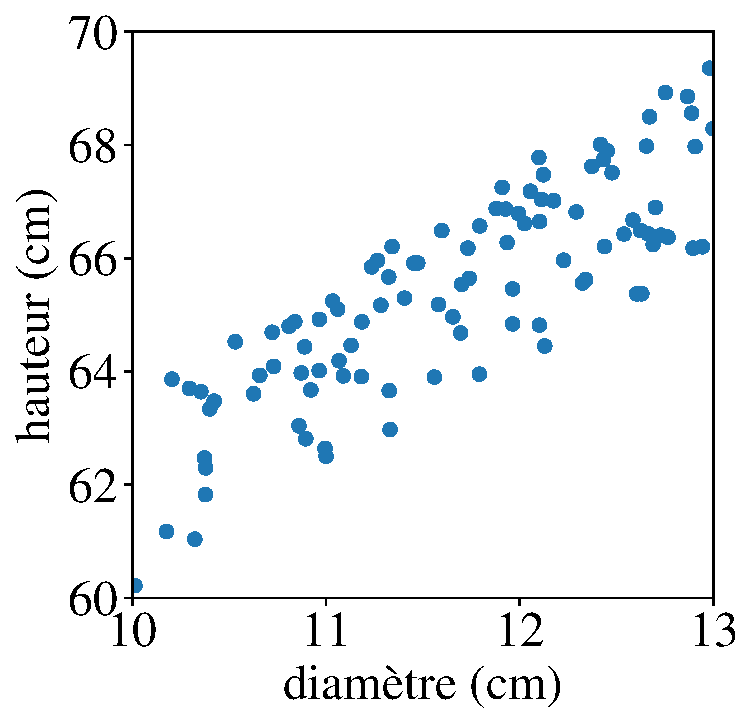
\includegraphics[width=0.35\textwidth]{figures/pearson_example}
\end{center}



\section*{Solution}
{%
	\noindent
	\rotatebox[origin=c]{180}{%
		\noindent
		\begin{minipage}[t]{\linewidth}
			\paragraph{Question 1.} Une série de boîtes à moustaches est plus appropriée
			pour visualiser la relation entre une variable quantitative (durée du séjour)
			et une variable qualitative (âge par
			tranches). Cf. figure~\ref{fig:remboursement_rembourses_age}.\newline
			
			\paragraph{Question 2.} $r \approx 0,85.$ On peut voir à la « pente » que la
			corrélation est positive. La situation est intermédiaire entre celle des
			figures 2.6(\textsc{C}) $(r=0,50)$ et 2.6(\textsc{D}) $(r=1,00)$. Une
			corrélation de $0,95$ serait plus proche de la figure~\ref{fig:pearson}(\textsc{D}) que de
			celle donnée ci-dessus. Remarquez ici que les données ne sont pas homogènes, au
			sens où elles ont des échelles de valeurs différentes, contrairement à ce qui
			est représenté sur la figure~\ref{fig:pearson} ; cela ne change pas l'interprétation de la
			corrélation.
		\end{minipage}%
	}%
	
	
	%%% Local Variables:
	%%% mode: latex
	%%% TeX-master: "../../sdd_2025_poly"
	%%% End:
